
\section{Local connectivity and q-tameness} \label{s:connectivity}

Let $\H$ be a fixed partially exact homology theory.

\begin{defi} \label{defi:local_connectedness}
	For $n \in \Z$ a continuous map is said to be \textit{$n$-homologically small} ($\HS_n$) if the image of the map induced $\H_{n}$ is finitely generated.
	Furthermore, if the image is $0$ then we say it is \textit{$n$-homologically trivial} ($\HT_n$).
	The map is said to be \textit{$n$-homotopically trivial} $(\piT_{n})$ if the map induced by $\pi_{n}$ is 0.
	We omit references to $n$ if the conditions hold for all integers.
	The map is said to be \emph{null-homotopic} ($\NH$) if it is homotopic to a constant map.
% 	It is said to be $\piT$/$\HS$/$\HT$ if it is $\piT_{n}$/$\HS_n$/$\HT_n$ for every~$n$. 
\end{defi}

There are maps that are $\piT$ but not $\HT$ for say ordinary homology, an examples is the collapse of the 1-skeleton of the torus.
Naturally, $\HT$ does not imply $\piT$ either.
If the map is $\NH$ then it is $\piT$ and, if the value of $\H$ on a point is 0, $\HT$ as well.

\begin{defi}
	A space $X$ is said to be $\HLC$ (resp. $\piLC$, $\LC$) if for each $x \in X$ any neighborhood $V$ of $x$ contains a neighborhood $U$ of $x$ such that the inclusion $U \to V$ is $\HT$ (resp. $\piT$, $\NH$).
	%If the neighborhoods can be chosen so that these inclusion have contractible images we say that the space is \textit{locally contractible} ($\LC$).
\end{defi}

Local connectivity assumptions like the above ones have a long history of being used to ensure that different homology theories agree and to ensure that homology is finitely generated.
We mention the following examples of these two uses, recalling that a space is said to be \textit{paracompact} if every open cover has a locally finite open refinement, i.e., every point has a neighborhood intersecting finitely many sets in the refinement.

\begin{prop}[\citet{MR105677}] \label{prop:cech_sing_hom_hlc}
	\v{C}ech and singular homology with arbitrary coefficients coincide on the category of paracompact Hausdorff spaces which are $\HLC$ with respect to integral singular homology.
\end{prop}

\begin{prop}[{\citet[p.~109]{MR0007094}}]
	A compact $\piLC$ Hausdorff space has finite Betti numbers.
\end{prop}

%We will deduce the following similar result from our main contribution, \cref{t:strong local connectedness implies q-tameness}.

%\begin{prop} \label{prop:HLC_single_space}
%	Let $X$ be a compact Hausdorff space.
%	If $X$ is $\HLC$ then $\H_{n}(X)$ is finitely generated for all $n$.
%\end{prop}

As a direct consequence of the previous proposition, we obtain the following persistence result.

\begin{cor}
	Let $f \colon X \to \R$ be a function with compact sublevel set filtration. If every sublevel set is $\piLC$ then $\H (X_{\leq \bullet})$ is $\PFG$ in every degree, in particular q-tame.
\end{cor}

A similar statement with an $\HLC$ condition instead of the $\piLC$ conditions also holds as a consequence of our main theorem. Having each sublevel set being locally connected is, however, in many cases too restrictive.
We would like a relative condition for sublevel set filtrations to be sufficient to ensure the q-tameness of the associated persistence module.
% The following definitions are motivated by Morse's work, in particular his local connectivity conditions mentioned in the introduction and reviewed in \cref{s:surfaces}. 

\begin{defi} \label{defi:local_connectedness_filtrations}
	The sublevel set filtration of a function $f \colon X \to \R$ is said to be $\HLC$ (resp.\@ $\piLC$, $\LC$) if for any $\epsilon > 0$, $x \in X$, and $V$ an open neighborhood of $x$, there is a $\delta \in (0, \epsilon)$ and a neighborhood $U$ of $x$ with $U \subseteq V$ such that for every $c \geq 0$ the inclusion
	\begin{equation*}
	X_{\leq f(x) + c + \delta} \cap U \to X_{\leq f(x) + c + \epsilon} \cap V
	\end{equation*}
	is $\HT$ (resp.\@ $\piT$, $\NH$).
	We also consider a weaker version, referred to as \textit{weakly} $\HLC$ (resp. $\piLC$ and $\LC$), defined as above but with $c = 0$ fixed.
\end{defi}

% As for a single space, the $\LC$ notions imply the corresponding $\piLC$ notions and the corresponding $\HLC$ notions if $\H$ evaluated at a point is trivial.

We remark that Morse's 
% condition of the space $X$ being locally $f$-connected from
notion of local $f$-connectivity in \cite[p.431]{Morse.1940} that we quoted in the introduction is equivalent to the sublevel set filtration of $f$ being weakly $\piLC$.
The notion of $\piLC$ was also introduced by Morse, appearing three years earlier in \cite[p.421]{Morse.1937}.

We will now show that not even being weakly $\LC$ is enough to imply q-tameness in general.
To do so let us consider the \textit{$d$-dimensional Hawaiian earring}
\begin{equation*}
\HE = \bigcup_{n\in\mathbb{N}}\left\{(x_0,\dots,x_d)\in\R^{d+1} \ \middle | \ \left(x_0-\frac{1}{n}\right)^2+x_1^2+\dots+x_d^2=\left(\frac{1}{n}\right)^2\right\}.
\end{equation*}

\begin{figure}[t]
	\centering
	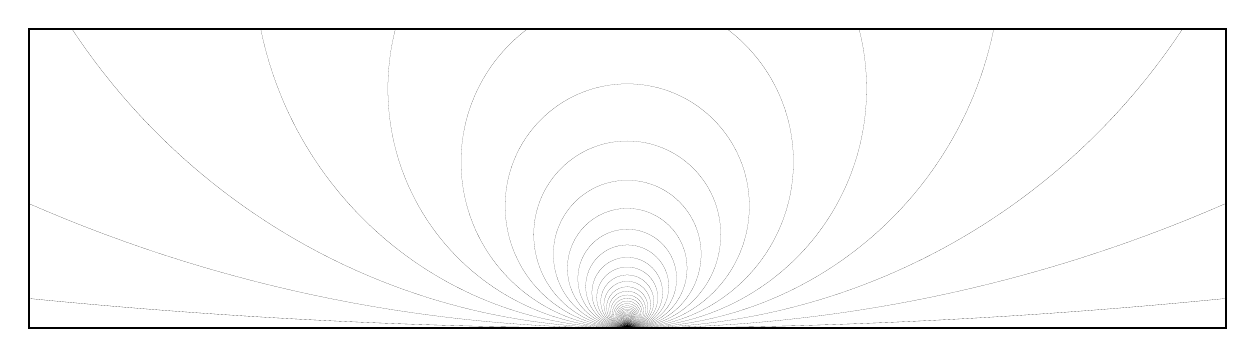
\begin{tikzpicture}[scale = 76]
	\draw[thick] (-.1,0) rectangle (.1,.05);
	\clip (-.1,0) rectangle (.1,.05); % remove for all circles
	\foreach \i in {1,...,100}{
		\draw[line width=0.1/\i mm] (0, 1/\i^2) circle (1/\i^2);
	}
	\end{tikzpicture}
	\caption{A closeup of the Hawaiian earring $\mathbb{H}^1$.}
	\label{fig:earrings}
\end{figure}

\begin{thm} \label{thm:counterexample}
	The function $f \colon \HE \to \R$ whose value at the origin is $0$ and is $1$ everywhere else defines a weakly $\LC$ compact sublevel set filtration that is not q-tame with respect to $\H$ if $\H_{n}(\HE)$ is not finitely generated for some $n$.
\end{thm}

\begin{proof}
	The space $\HE$ is Hausdorff and locally compact since $\R^{d+1}$ is.
	To verify that $f$ has compact sublevel sets we notice that all level sets are either the empty set, the singleton containing the origin, or $\HE$ itself, all compact spaces.
	Let us now verify that the sublevel set filtration of $f$ is weakly $\LC$.
	Let $\epsilon > 0$ and $x \in \HE$.
	If $x$ is the origin, we choose $\delta$ between $0$ and the minimum of $\epsilon$ and $1$.
	Then $\HE_{\leq f(x) + \delta} = \HE_{\leq \delta} = \{x\}$, so the weak $\LC$ condition is trivially satisfied.
	For $x$ not the origin, there is a unique $d$-sphere in $\HE$ that contains it.
	Clearly, we may choose $\delta > 0$ so small that $D_\delta(x) = \{y \in \R^{d+1} \mid \Vert x - y \Vert < \delta\} \cap \HE$ is a disk contained in this sphere, so $D_\delta(x)$ can be contracted to $\{x\}$ and the weak $\LC$ condition again follows trivially.
	What remains to be shown is that $\HE_{\leq \bullet}$ is not q-tame for $\H$. This follows directly from our assumption that $\H_{n}(\HE)$ is not finitely generated for some $n$ because $\HE_{\leq t}$ is constant with value $\HE$ for $t \geq 1$.
\end{proof}

The homology theories that we are most interested in do satisfy the condition in the previous theorem.

\begin{prop}
	There is an $n$ such that $\H_{n}(\HE)$ is not finitely generated if $\H$ is singular homology with arbitrary coefficients or \v{C}ech homology with field coefficients.
\end{prop}

\begin{proof}
	Both assertions are well-known. The case singular homology can be found in \cite{Barratt.1962}. For the reader's convenience, we present the \v{C}ech homology case.
	One can use the fact that it commutes with totally ordered limits for compact Hausdorff spaces \cite[Theorems VIII.3.6.\@ and X.3.1.]{MR0050886}:
	Define 
	\begin{align*}
	\HE_k &= \left\{ (x_0, \dots, x_d) \in \R^{d+1} \ \middle|\  \left( x_0 - \frac{1}{k} \right)^2 + x_1^2 + \dots + x_d^2 \leq \left( \frac{1}{k} \right)^2 \right\} \\
	& \cup \bigcup_{n=1}^{k-1} \left\{ (x_0, \dots, x_d) \in \R^{d+1} \ \middle|\  \left( x_0 - \frac{1}{n} \right)^2 + x_1^2 + \dots + x_d^2 = \left( \frac{1}{n} \right)^2 \right \},
	\end{align*}
	i.e., the $d$-dimensional Hawaiian earring but with the $k$-th largest $d$-sphere filled.
	We have $\lim_{k} \HE_{k} = \bigcap_{k} \HE_{k} = \HE$, and hence $\CH_{d}(\HE; \mathbb{F}) = \lim_{k} \CH_{d}(\HE_{k}; \mathbb{F})$.
	Clearly, each $\HE_{k}$ is a CW-complex, so we can simply use cellular homology to compute
	\begin{equation*}
	\lim_{k}\CH_{d}(\mathbb{H}^{d}_{k})=\lim\left(\dots\to \prod_{n=1}^2\mathbb{F}\to \prod_{n=1}^1\mathbb{F}\to \prod_{n=1}^0\mathbb{F}\right)=\prod_{n\in\mathbb{N}}\mathbb{F},
	\end{equation*}
	which is infinite-dimensional over $\mathbb{F}$.
	This finishes the proof.
\end{proof}

In particular, this result invalidates the claim in \cite[Theorem 6.3]{Morse.1940} stating that weakly $\piLC$ implies q-tame with respect to \v{C}ech homology with field coefficients.

% After having shown the insufficiency of the weak conditions,
We will now show that for any homology theory the property of being $\HLC$ implies that of being q-tame for compact sublevel set filtrations.
Since the Douglas functional induces a filtration which is $\LC$, the following result fixes the gap in the Unstable Minimal Surface Theorem of Morse and Tompkins.

\begin{thm} \label{t:strong local connectedness implies q-tameness}
	Assume that $\H$ is \v{C}ech homology with field coefficients or that $\H$ is a homology theory such that there is some $n_0$ such that $\H_{n}$ is 0 for all $n \leq n_0$.
	If the sublevel set filtration of a function $f \colon X \to \R$ is compact and $\HLC$, then it is also q-tame.
\end{thm}

The general proof strategy is inspired by the proof of a result by Wilder as presented by Bredon \cite[Section II.17]{Bredon.1997}.
We collect the main ideas in three lemmas.

\begin{lem} \label{l:commutative algebra}
	Given a commutative diagram of modules over a principal ideal domain
	\begin{equation*}
	\begin{tikzcd}
	A_{1,1} \arrow[r] & A_{1,2} & \\
	A_{2,1} \arrow[r] \arrow[u] & A_{2,2} \arrow[r] \arrow[u] & A_{2,3} \\
	& A_{3,2} \arrow[r] \arrow[u] & A_{3,3} \arrow[u]
	\end{tikzcd}
	\end{equation*}
	where the middle row is exact and both $A_{2,1} \to A_{1,1}$ and $A_{3,3} \to A_{2,3}$ have finitely generated images, then so does $A_{3,2} \to A_{1,2}$.
\end{lem}

\begin{proof}
	This is proven via a straightforward diagram chase. For more details see \cite[Lemma 17.3]{Bredon.1997}.
\end{proof}

\begin{lem} \label{l:neighborhood third}
	Let $X$ be locally compact space.
	For any compact subset $K$ and open set $U$ with $K \subseteq U$ there exists a compact set $K^\prime$ such that
	\begin{equation*}
	K \subseteq \interior(K^\prime) \subseteq K^\prime \subseteq U.
	\end{equation*}
\end{lem}

\begin{proof}
	For any $x \in K$ choose a compact neighborhood $C(x) \subseteq U$.
	We have
	\begin{equation*}
	K \subseteq \bigcup_K \interior(C(x)) \subseteq \interior\left(\bigcup_K C(x)\right) \subseteq \bigcup_K C(x) \subseteq U
	\end{equation*}
	Since $K$ is compact, the first inclusion above is achieved over a finite subset $\{x_1, \dots, x_m\}$ of elements in $K$.
	Defining $K^\prime = \bigcup_{i=1}^m C(x_i)$ finishes the proof.
\end{proof}

\begin{lem} \label{l:key lemma for q-tameness}
    Let $\H$ and $f \colon X \to \R$ be as in \cref{t:strong local connectedness implies q-tameness}.
	Consider sets $C \subseteq L \subseteq X$ with $C$ compact and $L$ open.
	For any $s < t$ the inclusion
	\[C \cap X_{\leq s} \to L \cap X_{\leq t}\]
	is $\HS$.
\end{lem}

\begin{proof}
	We will prove a slightly stronger statement,
	that there is $\delta \in (0,\, t-s)$ such that the inclusion
	\[C \cap X_{\leq s+\delta} \to L \cap X_{\leq t}\]
	is $\HS_n$ for all $n$.
	The statement holds for $\HS_{n}$ in place of $\HS$ for any $n \leq n_0$ since $\H_{n}$ induces the zero map.
	We will proceed by induction on $n \geq n_0$
	assuming the statement for $\HS_{n-1}$. 
	
	As the first case, assume that $\H$ is a homology theory. Given an open subset $L \subseteq X$ and $s < t$, let $\Sigma_{s, t}$ be the collection of all 
% uli/max: simplified %	compact subsets $K \subseteq L$ for which there exists $\delta > 0$ 
% uli/max: simplified %	and an open neighborhood $U$ of $K$ with $K \subseteq U \subseteq L$ 
% uli/max: simplified %		such that the inclusion
% uli/max: simplified %	\[U \cap X_{\leq s+\delta} \to L \cap X_{\leq t}\]
    open subsets $V$ such that $\overline{V} \subseteq L$ is compact and
    has an open neighborhood $U$ with $\overline{V} \subseteq U \subseteq L$ 
    for which there exists $\delta > 0$ such that
    %such that for $V = \interior(K)$ 
    the inclusion
    \[U \cap X_{\leq s+\delta} \to L \cap X_{\leq t}\]
	is $\HS_n$.
	
% 	We start by showing that any point $x \in L \cap X_{\leq s}$ has a neighborhood in $\Sigma_{s, t}$.
% 	Consider an open neighborhood $U_x \subseteq L$ of $x$, and take $\epsilon > 0$ such that $s + \epsilon < t$.\todo{uli: this seems unnecessary. $U_x = L$ and $s + \epsilon = t$ might work already.}
% 	By the $\HLC$ of $(X,f)$ there is a $\delta \in (0, \epsilon)$ and an open neighborhood $W_x \subseteq U_x$ such that for $c = s - f(x)$ the following composition is $\HS$:
% 	\begin{equation*}
% 	W_x \cap X_{\leq f(x) + c + \delta} \to
% 	U_x \cap X_{\leq f(x) + c + \epsilon} \to
% 	L \cap X_{\leq t}.
% 	\end{equation*}
% 	By local compactness we can choose a compact neighborhood of $x$ contained in $W_x$.
% 	This proves the claim.
	
	We start by showing that any point $x \in L \cap X_{\leq s}$ has a neighborhood in $\Sigma_{s, t}$.
	Since the sublevel set filtration of $f$ is $\HLC$, there is a $\delta \in (0, t-s)$ and an open neighborhood $U_x \subseteq L$ such that the inclusion
	\begin{equation*}
	U_x \cap X_{\leq s + \delta} \to
	L \cap X_{\leq t}.
	\end{equation*}
	is $\HS$.
	By local compactness we can choose a compact neighborhood $K_x$ of $x$ contained in $U_x$. Now $V_x = \interior (K_x)$ is an open neighborhood of $x$ that is contained in $\Sigma_{s,t}$.
	This proves the claim.
	
	Next, we will show that the class $\Sigma_{s,t}$ is closed under finite unions.
	For $i \in \{1, 2\}$ let $V_i$ be in $\Sigma_{s,t}$ with $U_i$ and $\delta_i \in (0, t-s)$ 
% uli/max: simplified %		and $U_i$ open with $K_i \subseteq U_i \subseteq L$ 
% uli/max: simplified %			such that
% uli/max: simplified %		\[U_{i} \cap X_{\leq s+\delta_i} \to L \cap X_{\leq t}\]
%    and $V_i = \interior(K_i)$ 
    such that $\overline{V_i} \subseteq U_i \subseteq L$ and
	\[U_{i} \cap X_{\leq s+\delta_i} \to L \cap X_{\leq t}\]
	is $\HS_n$.
	Writing $K_i = \overline{V_i}$, we use \cref{l:neighborhood third} to construct compact sets $K_i^\prime$ such that
	\begin{equation*}
	K_i \subseteq \interior(K_i^\prime) \subseteq K_i^\prime \subseteq U_i.
	\end{equation*}
	Writing $V_i^\prime = \interior(K_i^\prime)$,
	we have 
	\begin{equation*}
	V_i \subseteq K_i \subseteq V_i^\prime 
	%\subseteq K_i^\prime 
    \subseteq U_i 
	\subseteq L.
	\end{equation*}
	Notice that for $\delta = \min_i\delta_i$ both inclusions
	\[V_i^\prime \cap X_{\leq s+\delta} \to L \cap X_{\leq t}\]
	are $\HS_n$.
	Additionally, the induction hypothesis implies that the inclusion
	\[
	K_1 \cap K_2 \cap X_{\leq s} \to V_1^\prime \cap V_2^\prime \cap X_{\leq s+\delta}
	\]
	is $\HS_{n-1}$, and thus so is the inclusion
	\[
	V_1 \cap V_2 \cap X_{\leq s} 
% 	\to K_1 \cap K_2 \cap X_{\leq s} 
	\to V_1^\prime \cap V_2^\prime \cap X_{\leq s+\delta}.
	\]
    Because the $V_i$ and $V_i'$ are open and because $\H$ is a homology theory, we can use Mayer-Vietoris sequences to obtain the following commutative diagram satisfying the assumptions of \cref{l:commutative algebra}:
	\begin{equation*}
	\begin{tikzcd}[column sep=small]
	\H_n(L \cap X_{\leq t}) \oplus \H_n(L \cap X_{\leq t}) \arrow[r] &
	\H_n(L \cap X_{\leq t}) & \\
	\H_{n}(V_1^\prime \cap X_{\leq s+\delta}) \oplus \H_n(V_2^\prime \cap X_{\leq s+\delta}) \arrow[r] \arrow[u] & 
	\H_{n}((V_1^\prime \cup V_2^\prime) \cap X_{\leq s+\delta}) \arrow[r] \arrow[u] &
	\H_{n-1}(V_1^\prime \cap V_2^\prime \cap X_{\leq s+\delta}) \\ & 
	\H_{n}((V_1 \cup V_2) \cap X_{\leq s}) \arrow[r] \arrow[u] &
	\H_{n-1}(V_1 \cap V_2 \cap X_{\leq s}). \arrow[u]
	\end{tikzcd}
	\end{equation*}
	We conclude that $V_1 \cup V_2 \in \Sigma_{s, t}$.
	
	In the second case where $\H$ is \v{C}ech homology with field coefficients, the conditions for Mayer-Vietoris are different, so we also want a different definition of $\Sigma_{s,t}$. Concretely, in this case, let $\Sigma_{s, t}$ be the collection of all compact subsets $K$ of $L$ for which there exists $\delta_K > 0$ and an open neighborhood $U(K) \subseteq L$ of $K$ such that the inclusion $U(K) \cap X_{\leq s+\delta_K} \to L \cap X_{\leq t}$ is $\HS_n$.
	
	Again, we show that any point $x \in L \cap X_{\leq s}$ has a neighborhood in $\Sigma_{s, t}$.
	Take $\epsilon > 0$ such that $s + \epsilon < t$.
 	Since $L$ is open and the sublevel set filtration of $f$ is $\HLC$ is a $\delta \in (0, \epsilon)$ and an open neighborhood $W_x \subseteq L$ such that for $c = s - f(x)$ the inclusion 
 	\begin{equation*}
 	W_x \cap X_{\leq f(x) + c + \delta} \to
 	L \cap X_{\leq t}
 	\end{equation*}
 	is $\HS$.
 	By local compactness of $X$ we can choose a compact neighborhood of $x$ contained in $W_x$.
 	This proves the claim.
 	
 	Next, we will show that also in the \v{C}ech case, $\Sigma_{s,t}$ is closed under finite unions.
 	For $i \in \{1, 2\}$ let $K_i$ be in $\Sigma_{s,t}$ with $\delta_i > 0$ and $U_i \supseteq K_i$ open such that $U_{i} \cap X_{\leq s+\delta_i} \to L \cap X_{t}$ is $\HS_n$.
	We use \cref{l:neighborhood third} to construct sets $K_i^\prime$ such that
	\begin{equation*}
	K_i \subseteq \interior(K_i^\prime) \subseteq K_i^\prime \subseteq U_i.
	\end{equation*}
	Notice that for $\delta = \min(\delta_i)$ we have $K_i^\prime \cap X_{\leq s+\delta} \to L \cap X_t$ is $\HS_n$.
	Additionally, the induction hypothesis implies that $K_1 \cap K_2 \cap X_{\leq s} \to K_1^\prime \cap K_2^\prime \cap X_{\leq s+\delta}$ is $\HS_{(n-1)}$.
	Because the $K_i$, $K_i'$ and the sublevel sets of $f$ are conpact Hausdorff, we can use Mayer-Vietoris sequences to obtain the following commutative diagram satisfying the assumptions of \cref{l:commutative algebra}:
	\begin{equation*}
	\begin{tikzcd}[column sep=small]
	\H_n(L \cap X_{\leq t}) \oplus \H_n(L \cap X_{\leq t}) \arrow[r] &
	\H_n(L \cap X_{\leq t}) & \\
	\H_{n}(K_1^\prime \cap X_{\leq s+\delta}) \oplus \H_n(K_2^\prime \cap X_{\leq s+\delta}) \arrow[r] \arrow[u] & 
	\H_{n}((K_1^\prime \cup K_2^\prime) \cap X_{\leq s+\delta})) \arrow[r] \arrow[u] &
	\H_{n-1}(K_1^\prime \cap K_2^\prime \cap X_{\leq s+\delta}) \\ & 
	\H_{n}((K_1 \cup K_2) \cap X_{\leq s}) \arrow[r] \arrow[u] &
	\H_{n-1}(K_1 \cap K_2 \cap X_{\leq s}). \arrow[u]
	\end{tikzcd}
	\end{equation*}
	We conclude that $K_1 \cup K_2 \in \Sigma_{s, t}$.
	
	We can now finish in both cases simultaneously: Since any point in $L$ has a neighborhood in $\Sigma_{s,t}$, the set $C \subseteq L$ can be covered by sets in $\Sigma_{s,t}$. As $C$ is compact, this cover can be chosen finite. This implies the induction step because $\Sigma_{s,t}$ is closed under finite unions, so the lemma is proven.
\end{proof}

We can now complete the proof of the claim stating that for compact sublevel set filtrations, $\HLC$ implies q-tameness. 
\begin{proof}[Proof of \cref{t:strong local connectedness implies q-tameness}]
	This follows from applying \cref{l:key lemma for q-tameness} with $C = X_{\leq s}$ and $L = X$.
\end{proof}

